\documentclass{beamer}

\usepackage{beamerthemesplit}

\usecolortheme{seahorse}
\useinnertheme{rectangles}
\setbeamertemplate{footline}[frame number]

\title{\small{Combining Sketch and Tone for Pencil Drawing Production}}
\author{Stefan Burnicki, Raphael Braun, Andreas Altergott}
\date{\today}

\begin{document}
    \frame{\titlepage}

    \section{Introduction}
      \subsection{Spoiler}
        \frame{
            \frametitle{Spoiler}
            \begin{figure}[htbp]
                \centering
                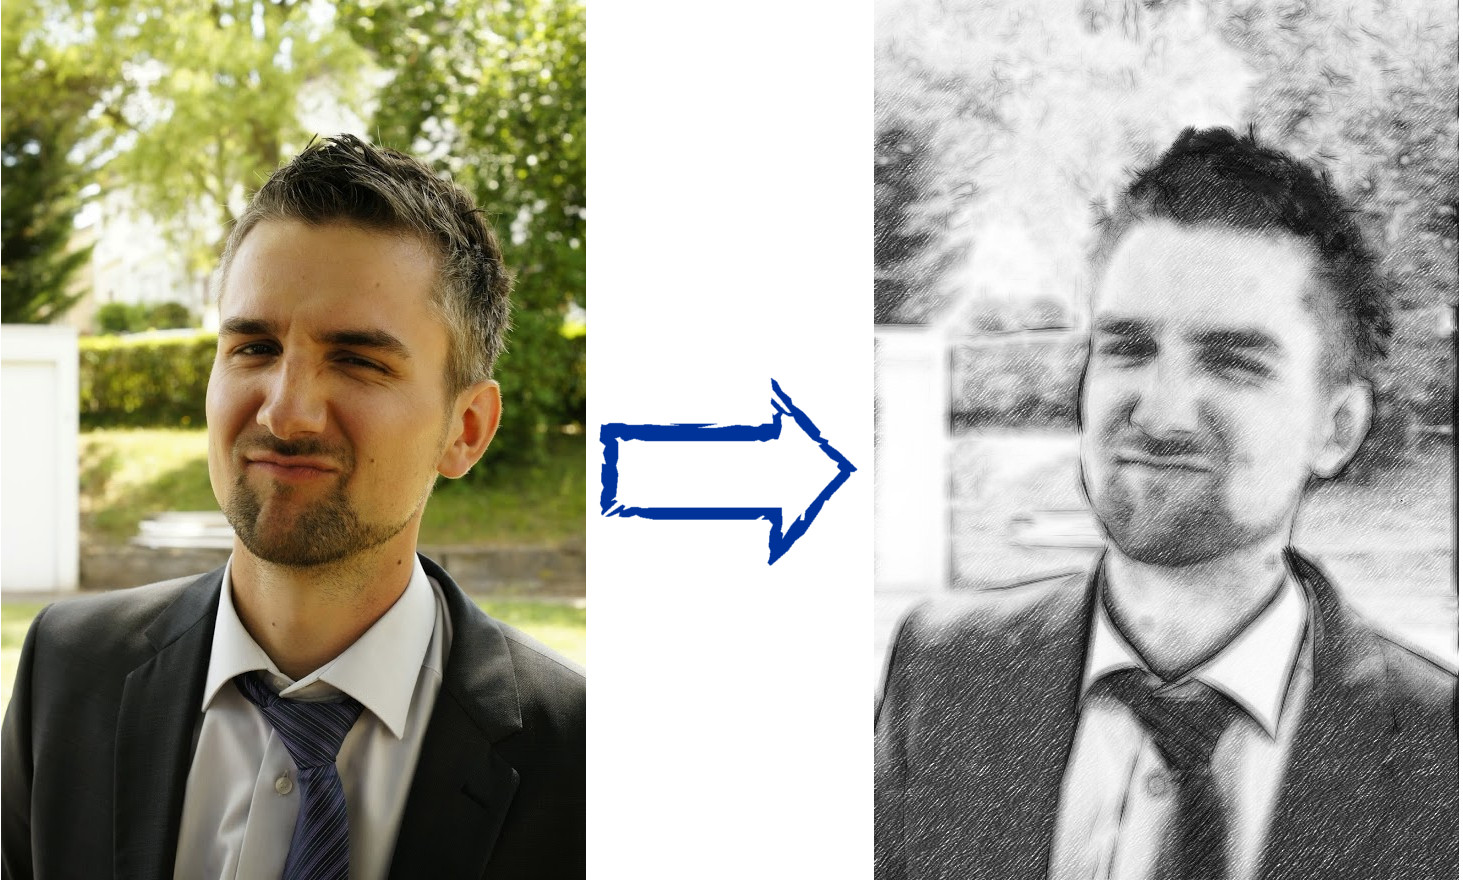
\includegraphics[scale = 0.2]{img/spoiler.jpg}
            \end{figure}
        }
      \subsection{Table of Contents}
        \frame{
            \frametitle{Table of Contents}
            \tableofcontents
        }
      \subsection{Project Objectives}
        \frame{
        	\frametitle{Project Objectives}
            \begin{itemize}
            	\item GPU implementation of the paper Combining Sketch and Tone for Pencil Drawing Production
                \item GPU implementation must be faster than the CPU implementation
                \item Understanding of a larger CUDA implementation
            \end{itemize}
        }
      \subsection{Implementation Steps}
        \frame{
        	\frametitle{Implementation Steps}
            \begin{figure}[htbp]
                \centering
                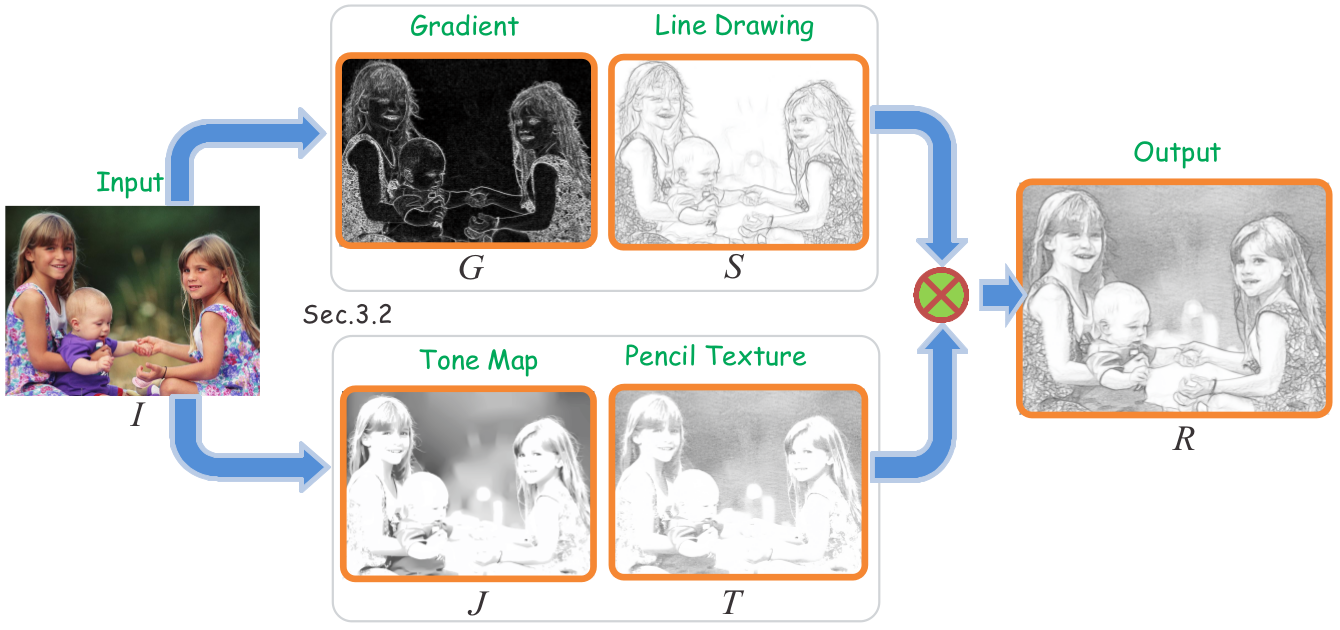
\includegraphics[scale = 0.15]{img/overview.png}
                \caption{Overview of the pencil drawing framework}
            \end{figure}
            \begin{itemize}
            	\item Line Drawing
                \item Tone Drawing
                \item Merge of Line and Tone Drawing
            \end{itemize}
        }
    \section{Implementation}
      \subsection{Line Drawing}
        \frame{
        	\frametitle{Line Drawing}
            \begin{figure}[htbp]
                \centering
                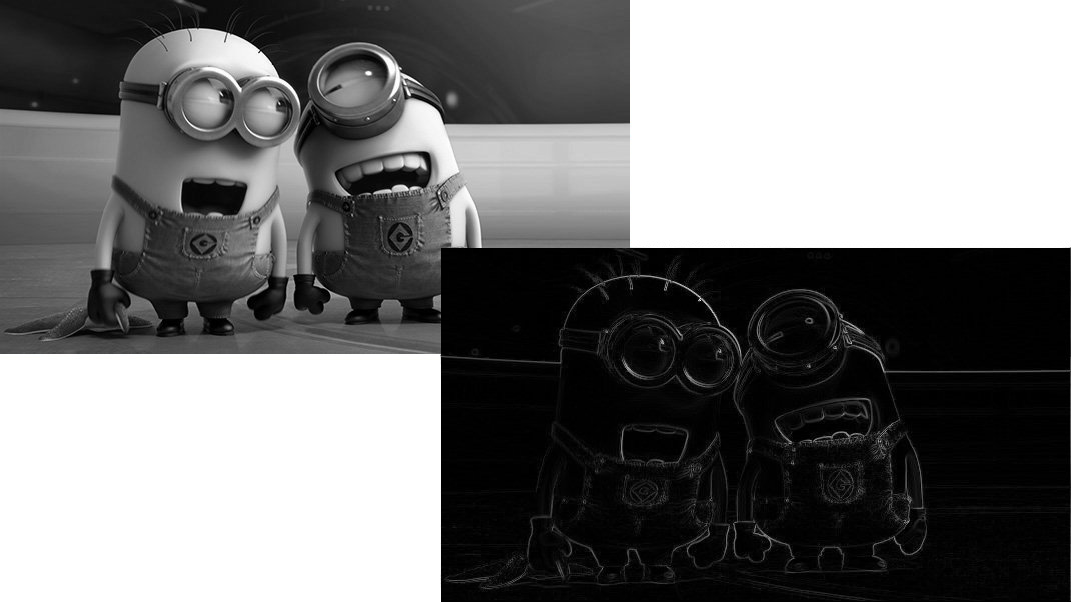
\includegraphics[scale = 0.2]{img/minions-1-gradient.png}
            \end{figure}
            \begin{itemize}
            	\item Forward gradient calculation on the gray-scale version of the image with $G = \left ( \left ( \partial_xI \right )^2 + \left ( \partial_yI \right )^2 \right )^{\frac{1}{2}}$
            \end{itemize}
        }
        \frame{
            \begin{figure}[htbp]
                \centering
                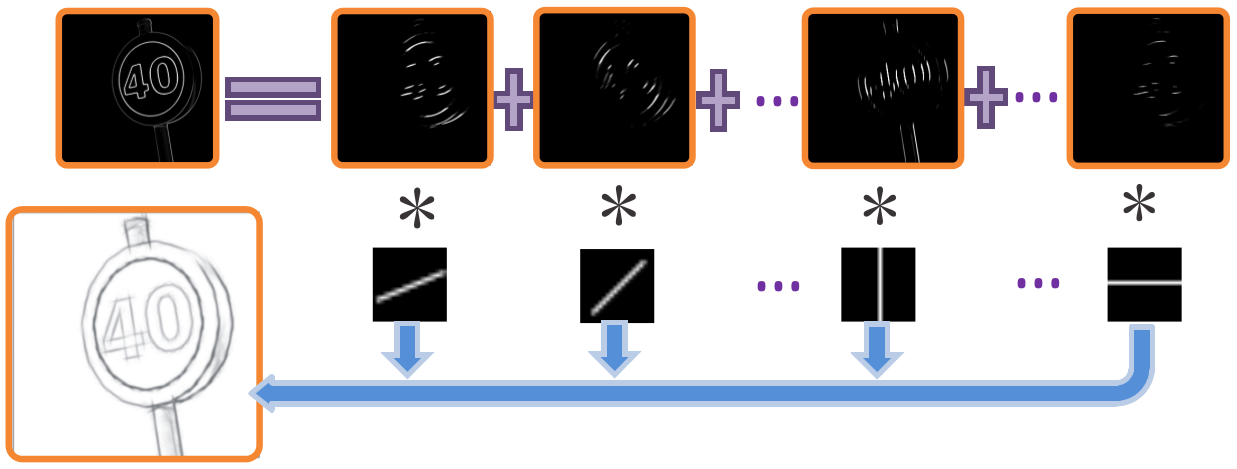
\includegraphics[scale = 0.2]{img/line_drawing.png}
                \caption{Line drawing with strokes}
            \end{figure}
            \begin{itemize}
                \item Computation of the response map with $G_i = L_i * G$, where $L_i$ is a line segment at direction $i$ (implemented in the convolution kernel) and $*$ the convolution operator
                \item Selection of the response for the pixel $p$ with the maximum value by $C_i \left ( p \right ) = \left \{ \begin{matrix} G \left ( p \right ) & if \: argmin_i \left \{ G_i \left ( p \right ) \right \} = i \\ 0 & otherwise \end{matrix} \right.$
            \end{itemize}
        }
        \frame{
            \begin{figure}[htbp]
                \centering
                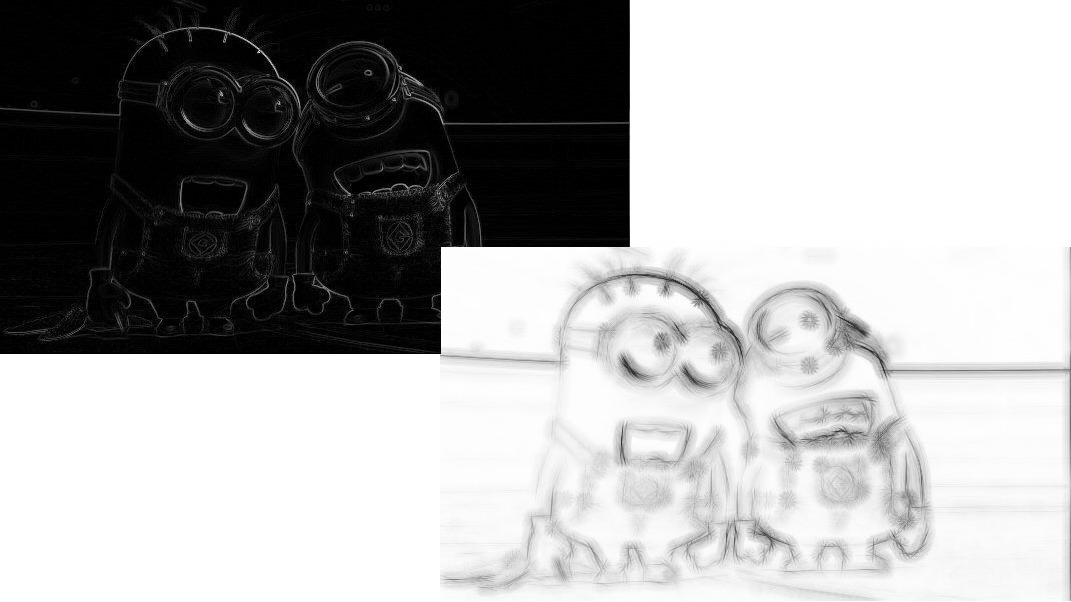
\includegraphics[scale = 0.2]{img/minions-2-convolution.png}
            \end{figure}
            \begin{itemize}
                \item Line Generation at each pixel with $S' = \sum \limits_{i = 1}^{8} \left ( L_i \otimes C_i \right )$
                \item Final stroke map $S$ obtained by inverting pixels of $S'$ and mapping them to $[0, 1]$
            \end{itemize}
        }
      \subsection{Tone Drawing}
        \frame{
            \frametitle{Tone Drawing}
            \begin{figure}[htbp]
                \centering
                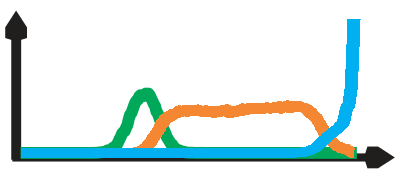
\includegraphics[scale = 0.2]{img/p123.png}
                \caption{Tone distribution $p_1, p_2, p_3$}
            \end{figure}
            \begin{itemize}
                \item Usage of constant parameters $\omega_1, \omega_2, \omega_3, \sigma_b, u_a, u_b, \mu_d, \sigma_d$
                \item Computation of distribution per tonal layer with $p \left ( v \right ) = \frac{1}{Z} \sum \limits_{i = 1}^3 \omega_i p_i \left ( v \right )$
                \item Computation of target tone distribution $p_1, p_2, p_3$ %with $p_1 \left ( v \right ) = \left \{ \begin{matrix} \frac{1}{\sigma_b} e^{-\frac{1 - v}{\sigma_b}} & if \: v \le 1 \\ 0 & otherwise \end{matrix} \right .$ $p_2 \left ( v \right ) = \left \{ \begin{matrix} \frac{1}{u_b - u_a} & if \: u_a \le v \le u_b \\ 0 & otherwise \end{matrix} \right .$ $p_3 \left ( v \right ) = \left \{ \begin{matrix} \frac{1}{\sqrt{2\pi\sigma_d}}e^{-\frac{\left ( v-\mu_d \right )^2}{2 \sigma_d^2}} & if \: u_a \le v \le u_b \\ 0 & otherwise \end{matrix} \right .$
                \item Pencil Texture rendering
            \end{itemize}
        }
        \frame{
            \begin{figure}[htbp]
                \centering
                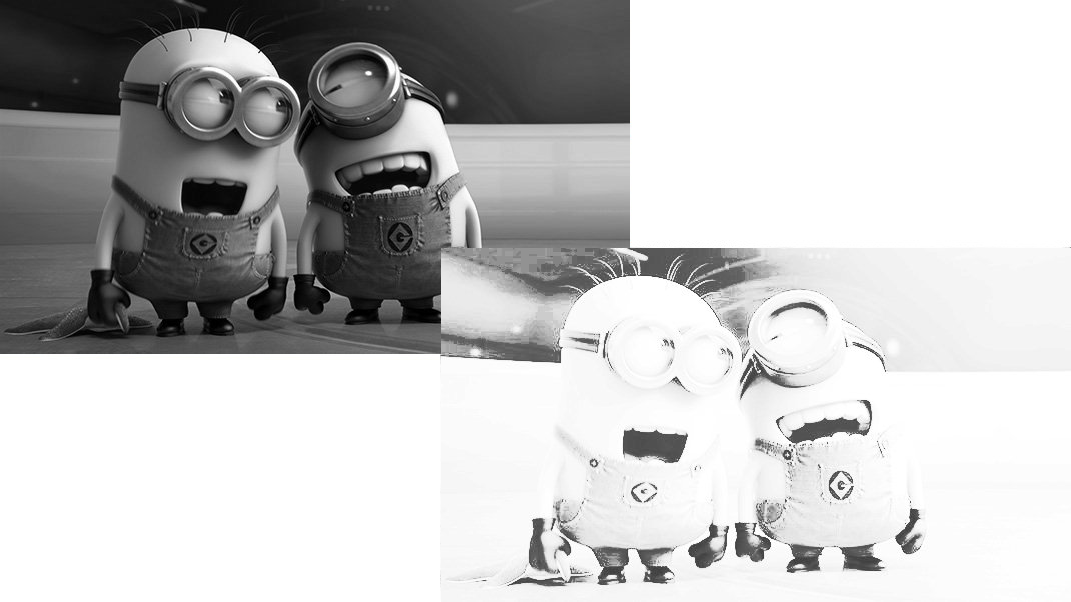
\includegraphics[scale = 0.2]{img/minions-3-tone.png}
                \caption{Result of tone map}
            \end{figure}
        }
        \frame{
            \begin{figure}[htbp]
                \centering
                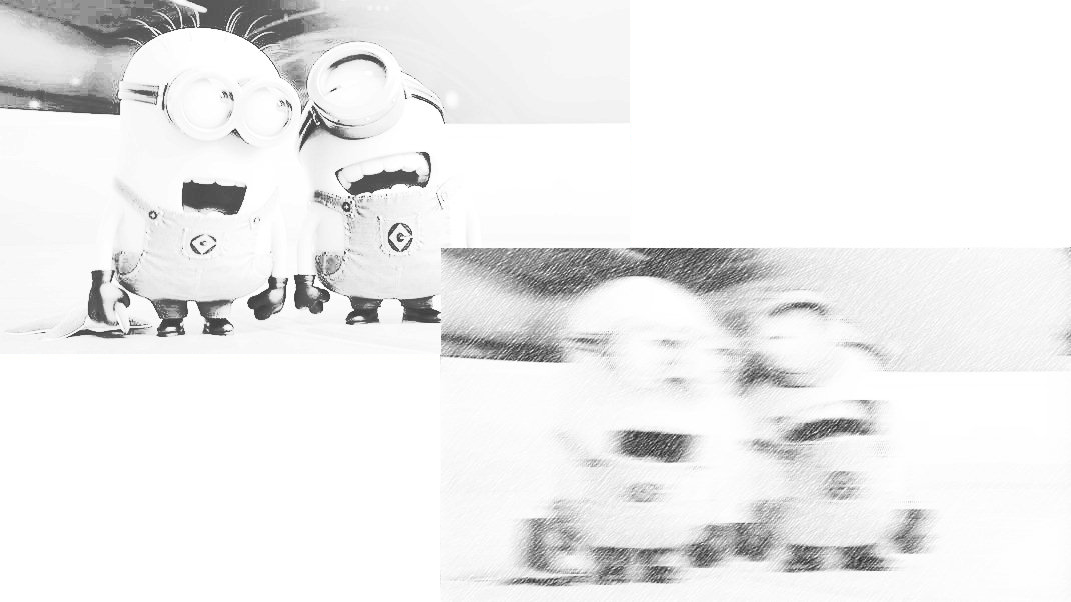
\includegraphics[scale = 0.2]{img/minions-4-potential.png}
            \end{figure}
            \begin{itemize}
                \item Pencil Texture rendering
            \end{itemize}
        }
      \subsection{Merge of Line and Tone Drawing}
        \frame{
            \frametitle{Merge of Line and Tone Drawing}
            \begin{figure}[htbp]
                \centering
                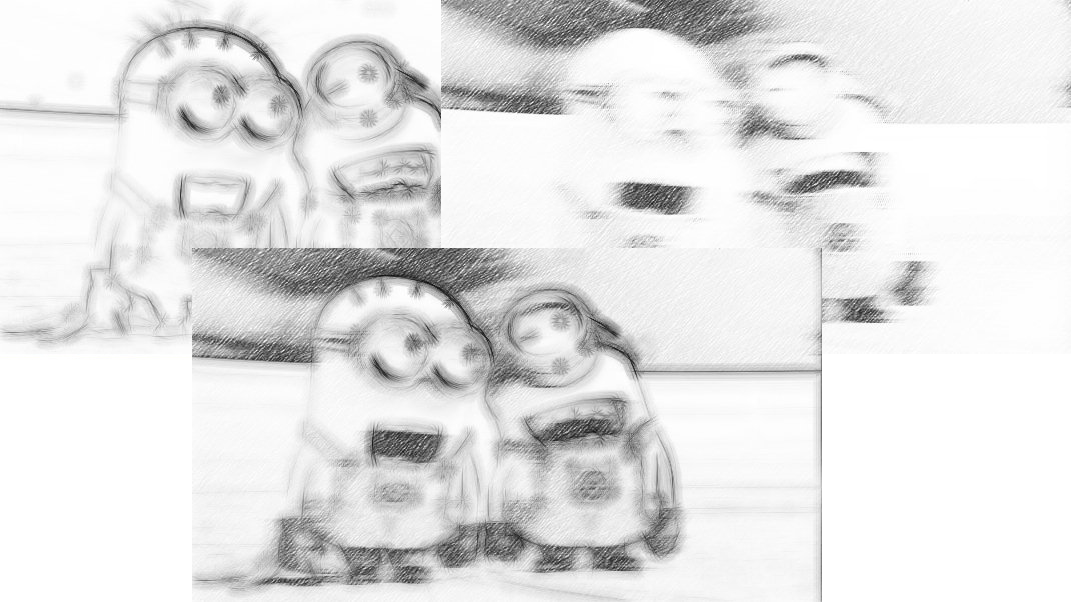
\includegraphics[scale = 0.2]{img/minions-5-multiplication.png}
            \end{figure}
            \begin{itemize}
                \item Multiplication of S and T values per pixel in $R = S \cdot T$
            \end{itemize}
        }
        \frame{
            \begin{figure}[htbp]
                \centering
                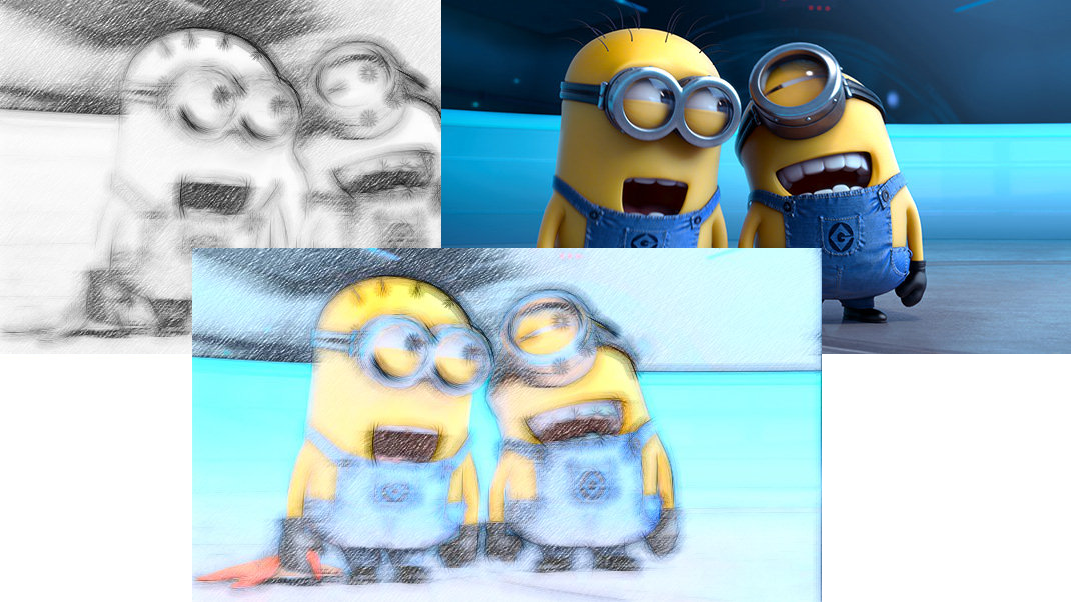
\includegraphics[scale = 0.2]{img/minions-6-coloring.png}
            \end{figure}
            \begin{itemize}
                \item Simply use generated output R as Y in YUV color space, keeping U and V from original image for colored output
            \end{itemize}
        }
      \subsection{Kernel Pipeline and Profiling}
        \frame{
            \frametitle{Kernel Pipeline}
            \begin{figure}[htbp]
                \centering
                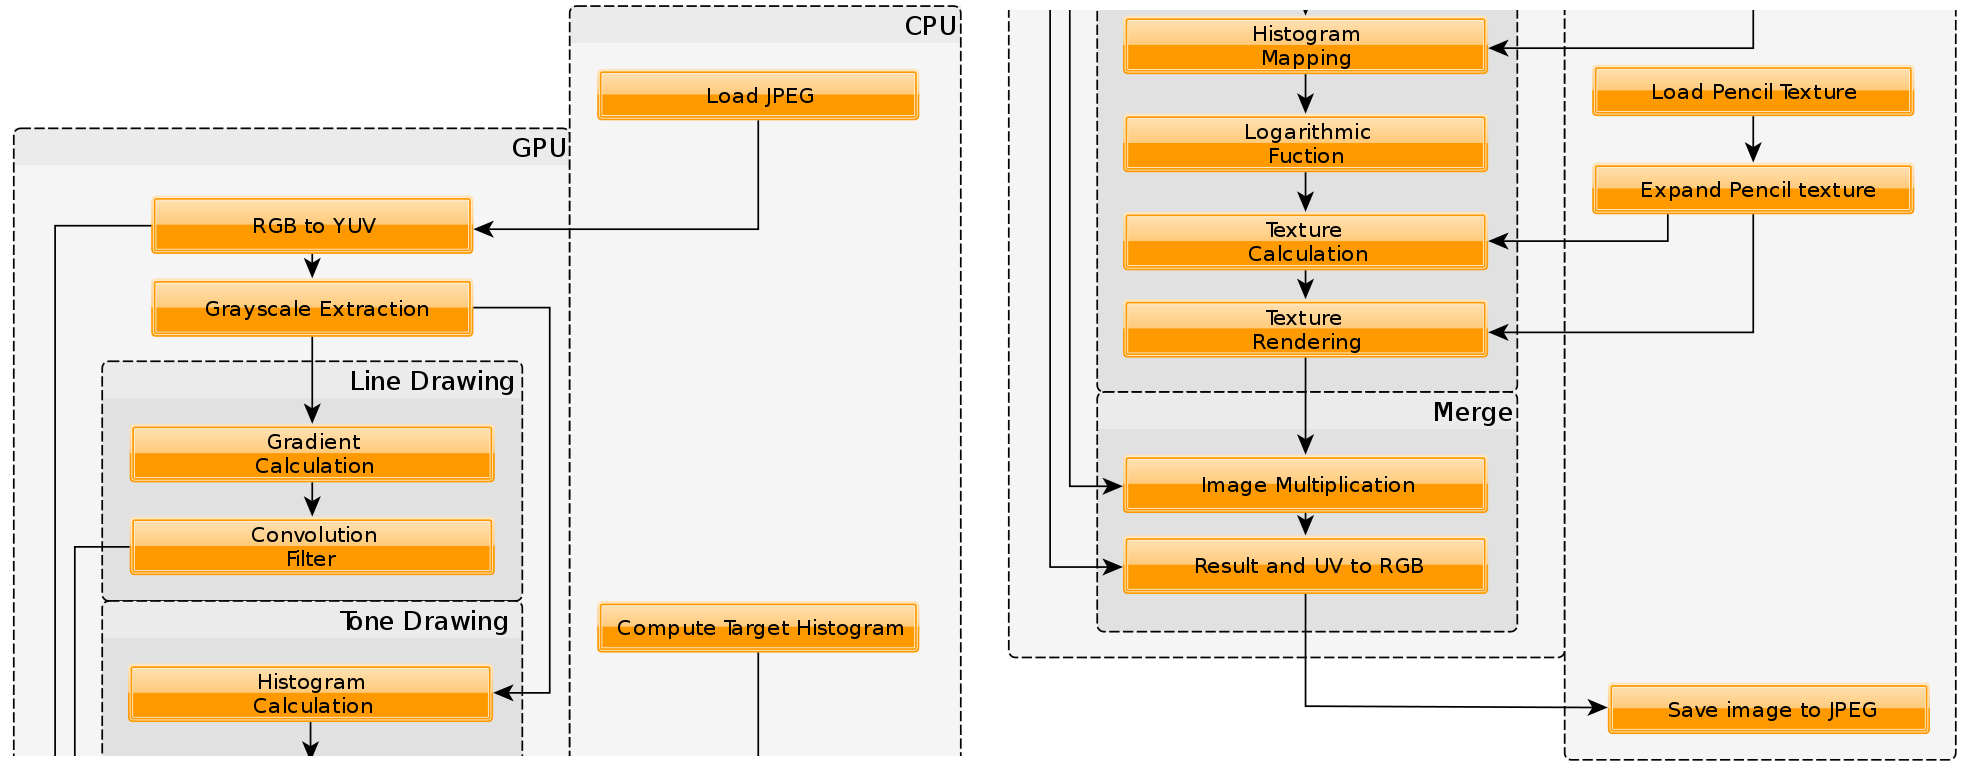
\includegraphics[scale = 0.28]{img/pipeline.png}
            \end{figure}
        }
    	\frame{
        	\frametitle{Profiling Results}
            \begin{figure}[htbp]
                \centering
                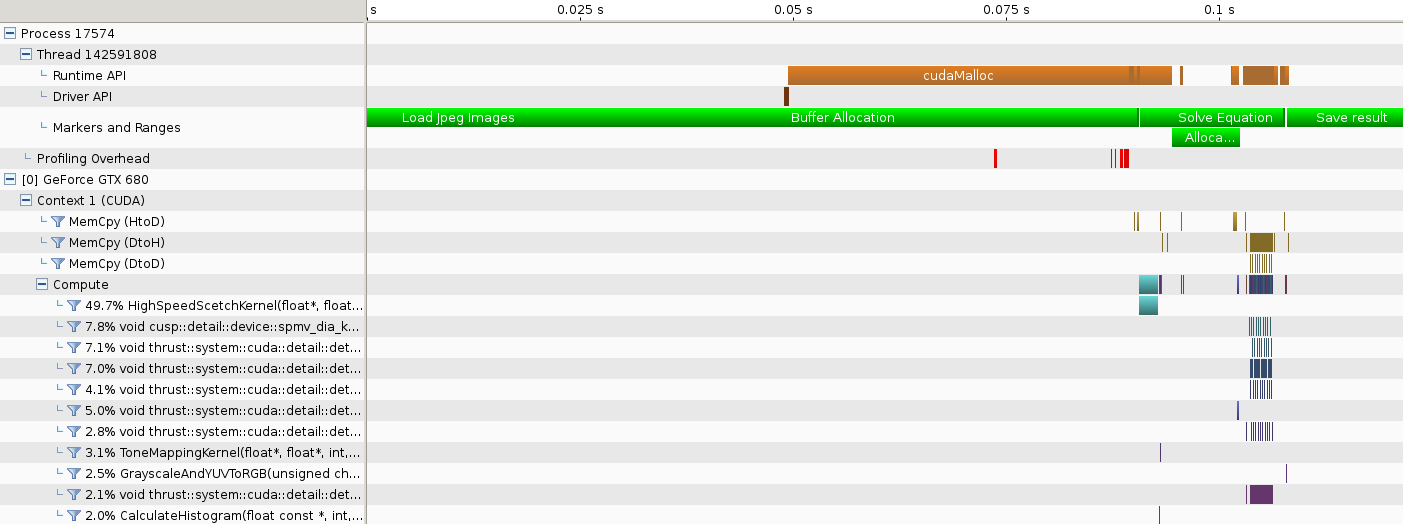
\includegraphics[scale = 0.35]{img/profiling_all.png}
            \end{figure}
        }
    \section{Live Demonstration}
        \frame{
            \frametitle{Live Demonstration}
            \begin{figure}[htbp]
                \centering
                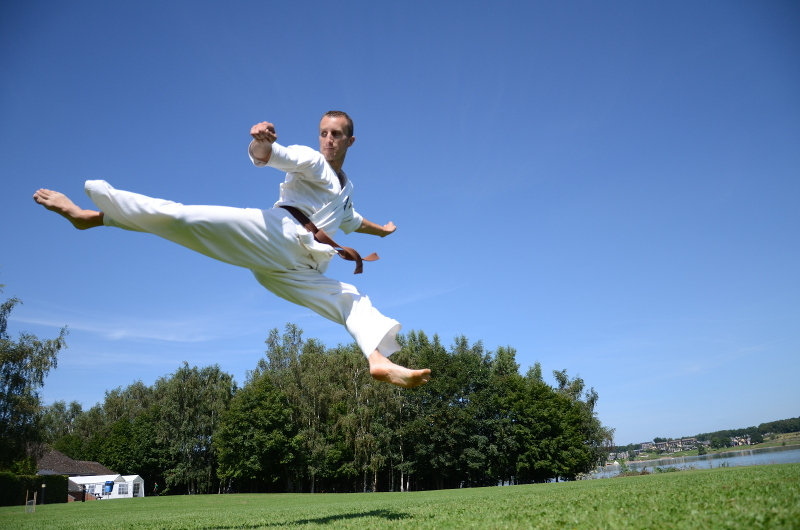
\includegraphics[scale = 1.4]{img/karate_jump.jpg}
            \end{figure}
        }
        \frame{
            \begin{figure}[htbp]
                \centering
                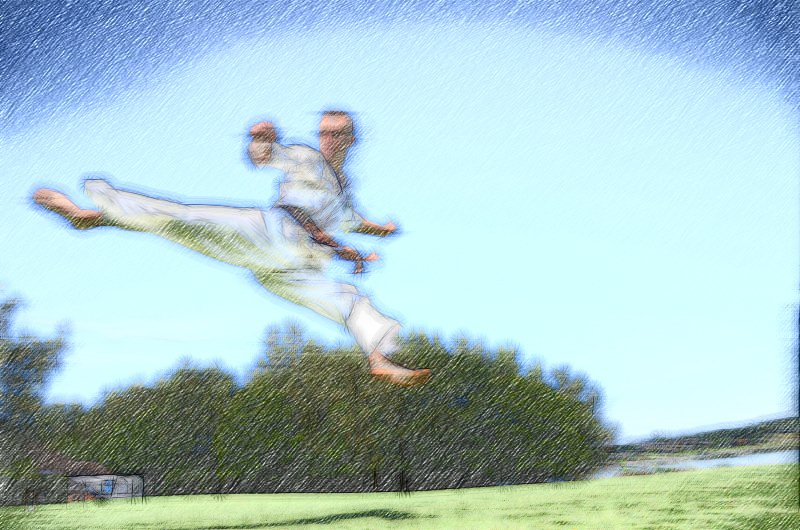
\includegraphics[scale = 0.38]{img/karate_jump-scetch.jpg}
            \end{figure}
        }
        \frame{
            \begin{figure}[htbp]
                \centering
                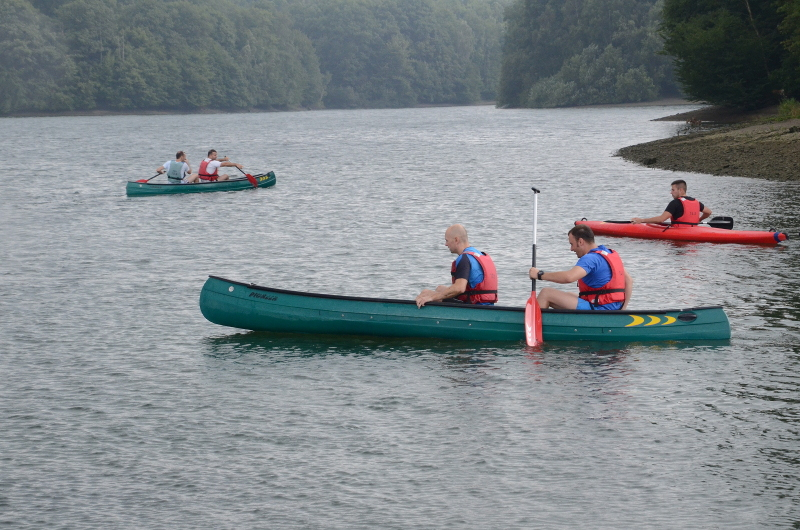
\includegraphics[scale = 1.58]{img/canoo.jpg}
            \end{figure}
        }
        \frame{
            \begin{figure}[htbp]
                \centering
                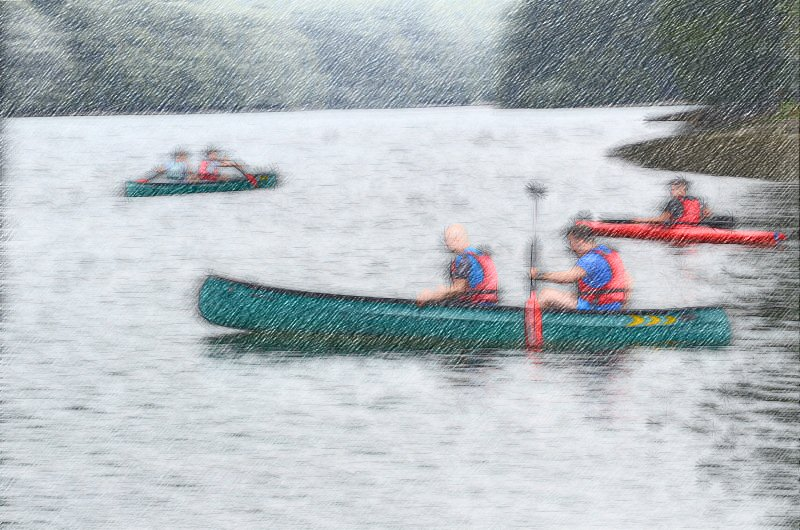
\includegraphics[scale = 0.38]{img/canoo-scetch.jpg}
            \end{figure}
        }
        \frame{
            \begin{figure}[htbp]
                \centering
                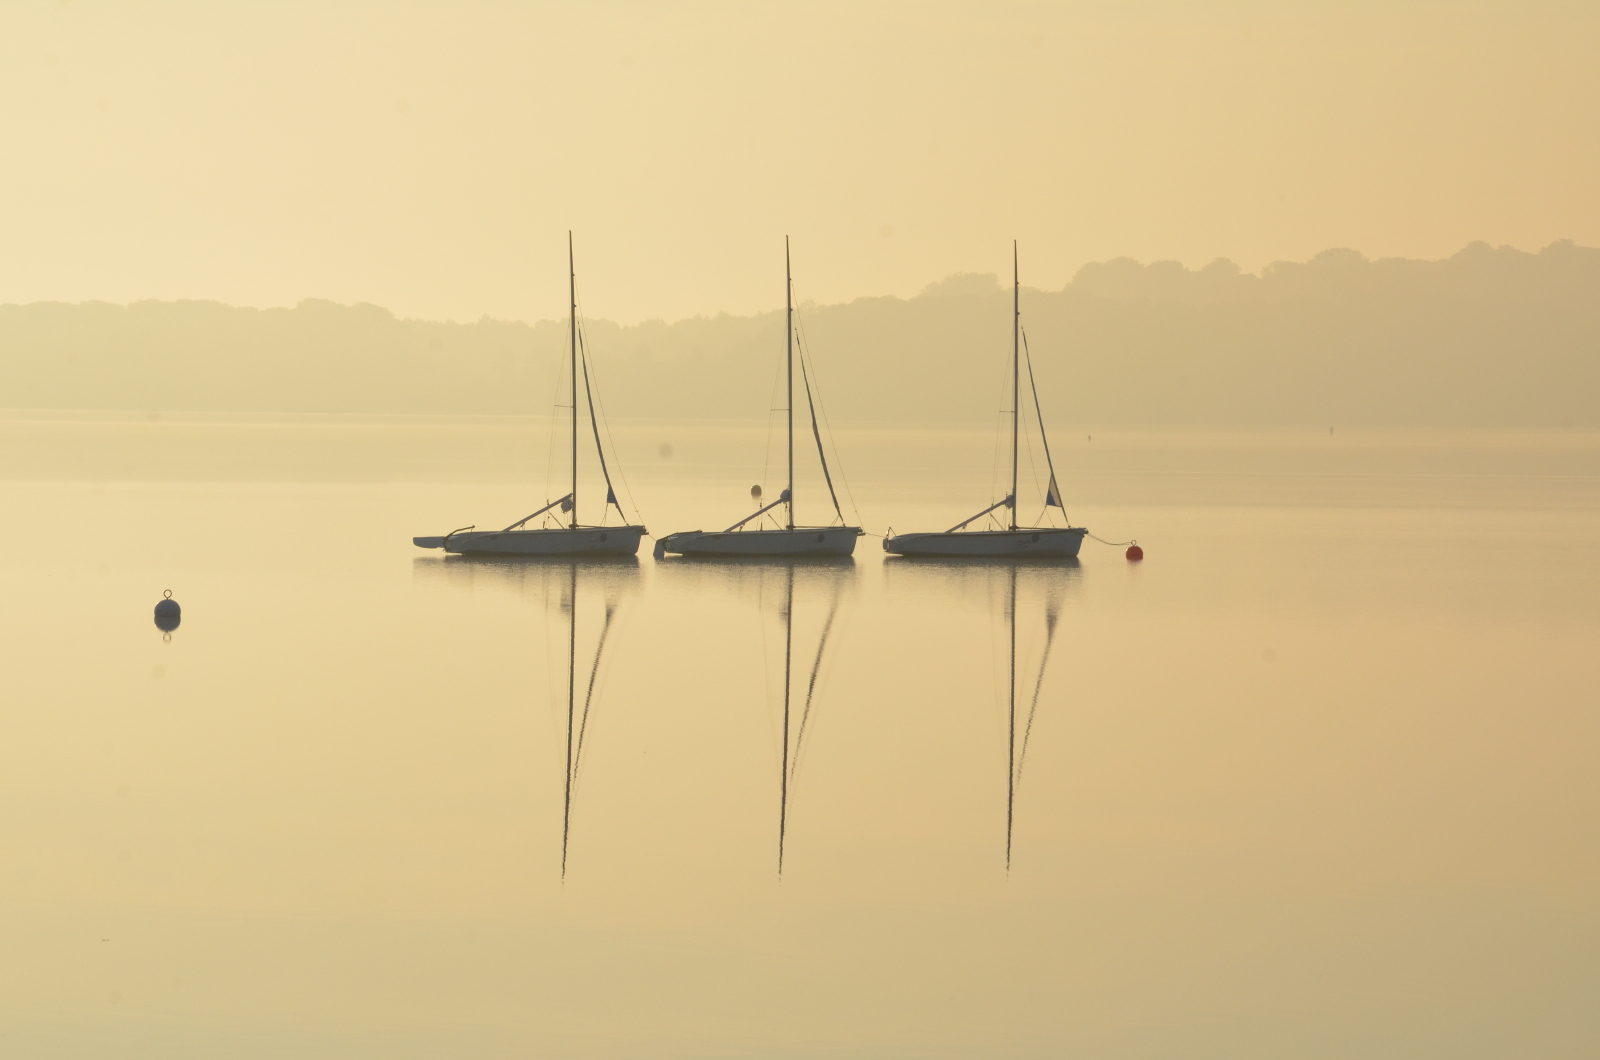
\includegraphics[scale = 0.78]{img/boats.jpg}
            \end{figure}
        }
        \frame{
            \begin{figure}[htbp]
                \centering
                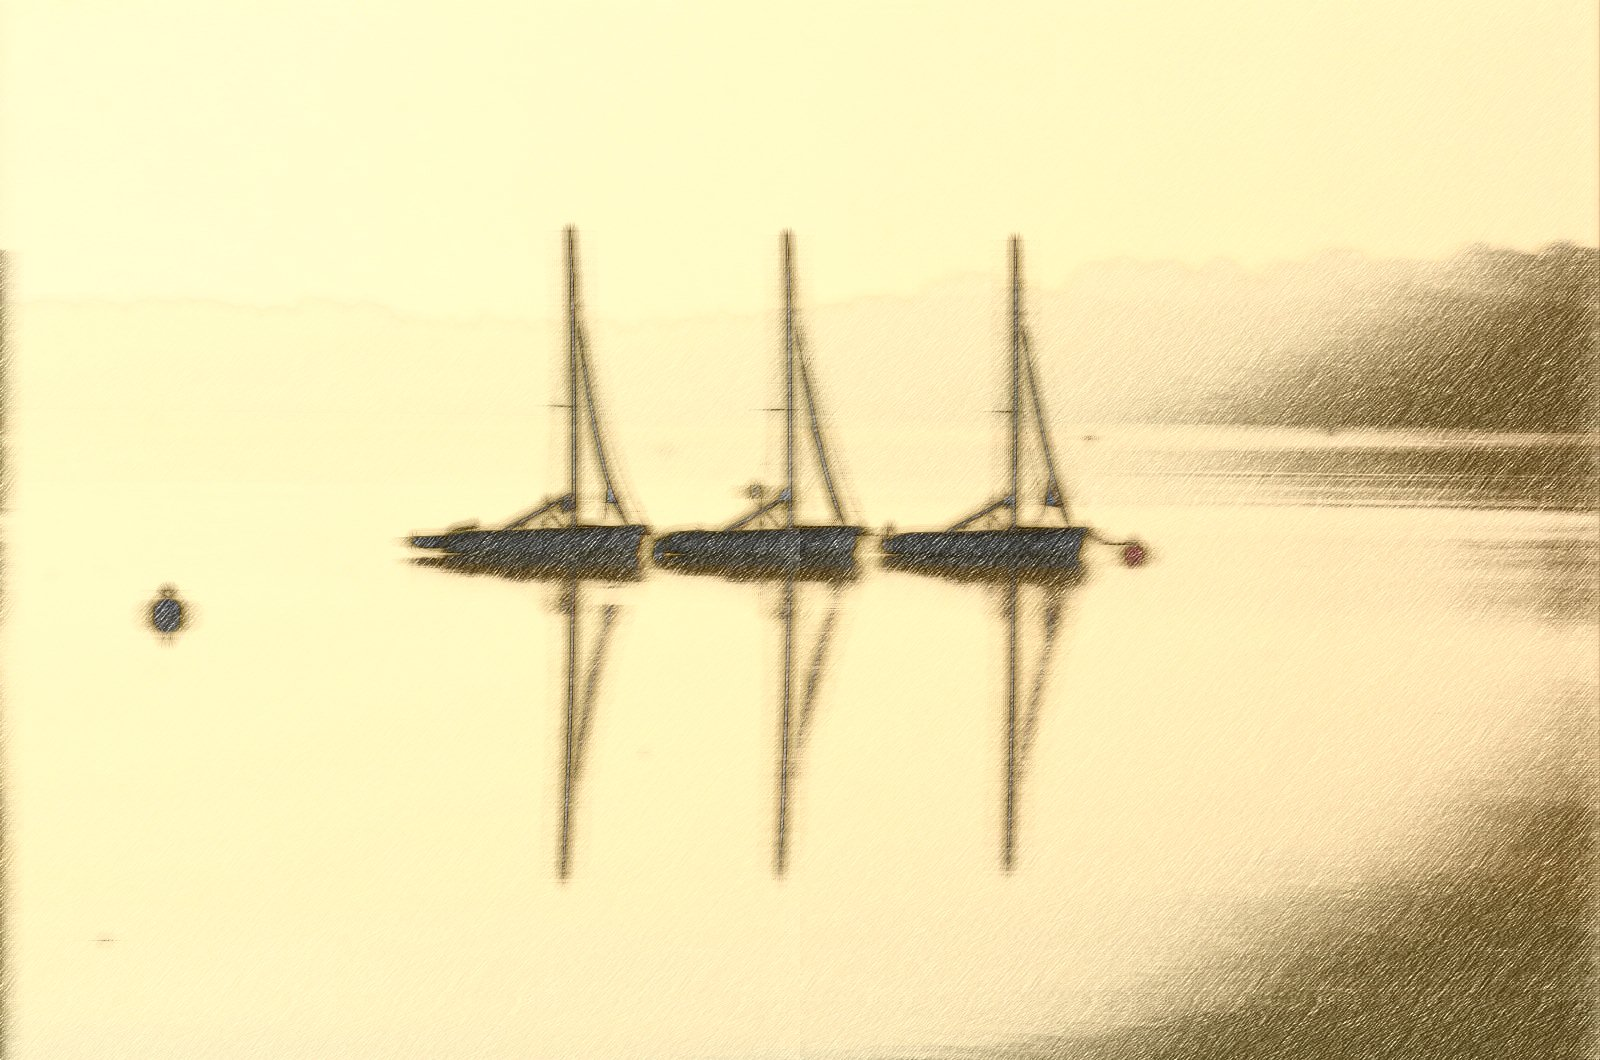
\includegraphics[scale = 0.19]{img/boats-scetch.jpg}
            \end{figure}
        }
    \section{Conclusion}
            \frame{
                \frametitle{Conclusion}
                \begin{itemize}
                    \item Successful GPU implementation of the sketch filter as described in the paper
                    % TODO: How much faster?
                    \item Our GPU implementation is faster than the version of the paper
                    \item Speedup of 72.1 compared to CPU implementation
                    of the original paper ($27.73 ms$ at $600 \times 600$ pixels)
                    \item 30 ms per frame in DVD quality
                    \item 60 ms per frame in HD Ready
                    \item 130 ms per frame in Full HD quality
                \end{itemize}
            }
            \frame{
            	\frametitle{Mastered Obstacles}
                \begin{itemize}
                	\item Understanding of the paper
                    \item Newcomers to image processing
                    \item Realization of a bigger GPU implementation
                \end{itemize}
            }
            \frame{
                \frametitle{Future Improvements}
                \begin{itemize}
                    \item Better optimization can improve performance even more
                    \item Pre image analyzer could automatically calculate the ideal line length for the line drawing
                    \item Pre image analyzer could also calculate the parameters for the tone drawing
                \end{itemize}
            }
            \frame{
                \begin{center}
                    Thank you for your attention.
                \end{center}
            }
            \frame{
                \begin{center}
                    Questions?
                \end{center}
            }
\end{document}
